\documentclass[10pt,a4paper,oneside]{article}
\usepackage[T1]{fontenc}
\usepackage[french]{babel}
\usepackage{textpos}
\usepackage{pstricks}
\usepackage{subfigure}
\usepackage{graphicx}
\usepackage{tikz}
\usepackage{fancyvrb}

\usetikzlibrary{shapes.geometric}
\usetikzlibrary{calc}
\usetikzlibrary{shadows}

\tikzstyle{every picture}=[scale=0.7, inner sep=1.5pt]
\def\des{\node[draw,shape=rectangle,rounded corners=2pt,minimum size=.5cm,shade]}

\usepackage[a4paper,hmargin=1.5cm, vmargin=1.5cm, centering]{geometry}

\begin{document}

\date{}
\author{}
\title{
    \vspace{-1.5cm}
    S U J E T\\
    {\Large \textsc{programmation événementielle : visual basic .net}}\\
    \vspace{3 mm}
    {\Large -- \textsc{Variante Du Jeu Mastermind} --}\\
}

\maketitle

\vspace{-2.1cm}

\section{Principe du jeu}
"Le {\em Mastermind} (ou Master Mind) est un jeu de société pour deux joueurs dont le but est de trouver un code. C'est un jeu de réflexion, et de déduction, inventé par Mordecai Meirowitz dans les années 1970 alors qu'il travaillait comme expert en télécommunications.

\medskip

Il se présente généralement sous la forme d'un plateau perforé de 10 rangées de quatre trous pouvant accueillir des pions de couleurs. Le nombre de pions de couleurs différentes est de 8 et les huit couleurs sont généralement : rouge ; jaune ; vert ; bleu ; orange ; blanc ; violet ; fuchsia. Il y a également des pions blancs et rouges (ou noirs) utilisés pour donner des indications à chaque étape du jeu. Il existe de nombreuses variantes suivant le nombre de couleurs, de rangées ou de trous.

\medskip

Un joueur commence par placer son choix de pions sans qu'ils soient vus de l'autre joueur à l'arrière d'un cache qui les masquera à la vue de celui-ci jusqu'à la fin de la manche. Le joueur qui n'a pas sélectionné les pions doit trouver quels sont les pions, c'est-à-dire leurs couleurs et positions. Pour cela, à chaque tour, le joueur doit se servir de pions pour remplir une rangée selon l'idée qu'il se fait des pions dissimulés. Une fois les pions placés, l'autre joueur indique le nombre de pions de la bonne couleur bien placés, ainsi que le nombre de pions de la bonne couleur mais mal placés.

\medskip

La tactique du joueur actif consiste à sélectionner en fonction des coups précédents, couleurs et positions, de manière à obtenir le maximum d'informations de la réponse du partenaire puisque le nombre de propositions est limité par le nombre de rangées de trous du jeu. Dans la plupart des cas, il s'efforce de se rapprocher le plus possible de la solution, compte tenu des réponses précédentes, mais il peut aussi former une combinaison dans le seul but de vérifier une partie des conclusions des coups précédents et de faire en conséquence la proposition la plus propice à la déduction d'une nouvelle information.

\medskip

Le joueur gagne cette manche s'il donne la bonne combinaison de pions sur la dernière rangée ou avant."

\begin{flushright}
    (source Wikipedia)
\end{flushright}

\section{Déroulement de l'application}

L'application débutera par le lancement d'un {\em formulaire d'accueil}. Ce formulaire présentera au minimum~:

\medskip

\begin{itemize}
  \item Deux {\em ComboBox} permettant de saisir le nom du premier et du second joueur. Une saisie dans une de ces {\em ComboBox} affichera la liste des joueurs déjà connus de l'application. Les deux joueurs ne devront pas pouvoir porter le même nom ;
  \item Un {\em Bouton} pour lancer la partie, une fois que les deux joueurs auront saisi un nom ;
  \item Un {\em Bouton} permettant de quitter l'application, à confirmer par une {\em MessageBox} ;
  \item Un {\em Bouton} lançant l'affichage du tableau des scores (voir section suivante).
\end{itemize}

\bigskip

Une fois la partie débutée, le premier joueur est invité à saisir une combinaison que le second joueur devra deviner. Afin de simplifier la programmation de ce projet, la combinaison à deviner ne sera pas composée de couleurs mais de 5 caractères spéciaux :

\begin{center}
    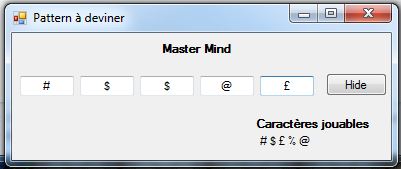
\includegraphics[scale=0.6]{pictures/player1.png}
\end{center}

Ce formulaire présentera 5 {\em TextBox} (chacune limitée à un seul des caractères autorisées) permettant au premier joueur de saisir sa combinaison. Un {\em Label} rappellera au joueur les caractères autorisés pour la saisie de cette combinaison. Le joueur peut utiliser plusieurs fois le même caractère pour composer sa combinaison.

\medskip

Une fois que les 5 caractères auront été saisis, un {\em Bouton} permettra de passer au formulaire suivant pour permettre au second joueur de tenter de deviner la combinaison. Ce joueur disposera alors de 15 coups et 1 min 30 pour atteindre ce but~:

\begin{center}
    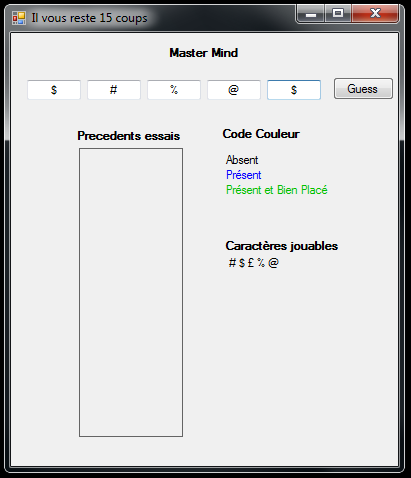
\includegraphics[scale=0.6]{pictures/player2try1.png}
\end{center}

Pour cela, ce formulaire présentera également 5 {\em TextBox} (limitées à un seul des caractères autorisées) permettant au second joueur de proposer une combinaison. Un {\em Label} rappellera également à ce joueur les caractères autorisés pour la saisie de sa proposition. A tout moment, des {\em labels} indiqueront au second joueur le nombre de propositions restantes ainsi que le temps restant pour deviner la combinaison.\\

Lorsque que les 5 caractères auront été saisis, un {\em Bouton} permettra au joueur de soumettre sa proposition~:

\begin{center}
    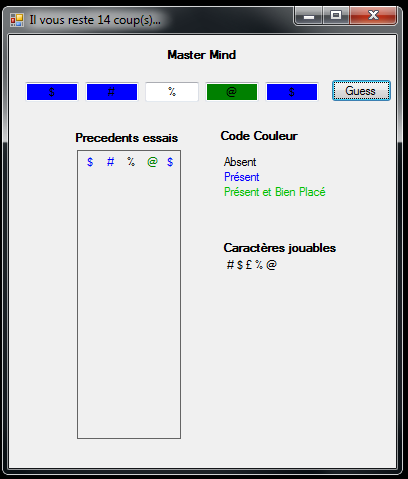
\includegraphics[scale=0.6]{pictures/player2try1answer.png}
\end{center}

Plutôt que d'informer le second joueur sur le nombre de caractère présents, bien ou mal placés, dans cette variante du Mastermind le jeu révélera directement le statut de chaque caractère proposé. Afin d'informer le second joueur, les {\em TextBox} utilisées pour la proposition emploieront un code couleur et indiqueront, pour chaque caractère proposé, si celui ci est présent et bien placé, présent mais mal placé ou absent de la combinaison à deviner. 

\medskip

Afin de garder un historique des coups précédent, chaque proposition du second joueur sera ajoutée dans un composant graphique de votre choix~:

\begin{center}
    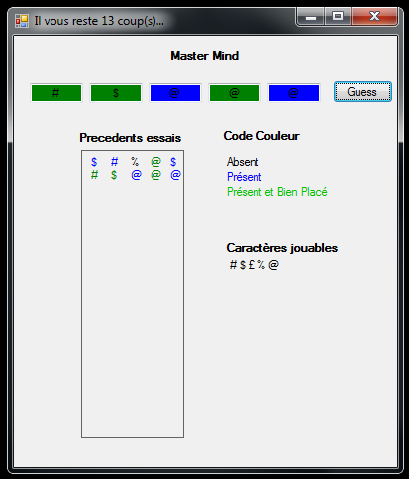
\includegraphics[scale=0.6]{pictures/player2try2answer.png}
\end{center}

Pour chacun des coups précédemment joués, l'historique devra afficher la réponse obtenue, précisant le statut de chaque caractère proposé à une position donnée.

\medskip

Le jeu se poursuit de la même façon jusqu'à ce que le second joueur devine la combinaison du premier joueur ou épuise les 15 propositions ou le temps imparti.

\begin{center}
    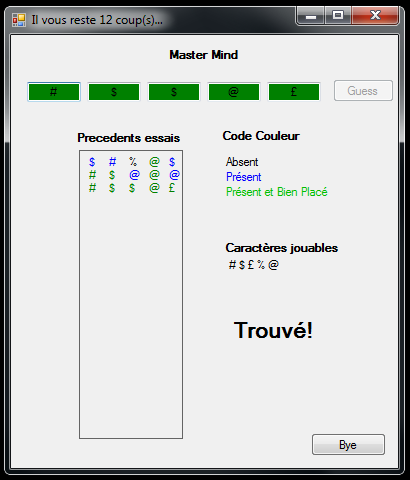
\includegraphics[scale=0.6]{pictures/player2victory.png}
\end{center}

A l'issue de la partie, le second joueur marque 1 point si il à réussi à deviner la combinaison. A l'inverse, le premier joueur marque 1 point si le second joueur n'est pas parvenu à deviner cette combinaison.

\medskip

Une fois la partie terminée, que le second joueur ait gagné ou perdu, un {\em Bouton} permettra de revenir au {\em formulaire d'accueil} qui proposera automatiquement la partie suivante. Les rôles seront alors inversés~: le nom du joueur ayant proposé la précédente combinaison apparait en second joueur (il devra alors tenter de deviner la nouvelle combinaison) ; celui du joueur ayant tenté de deviner la combinaison précédente apparaît en premier joueur (il devra cette fois ci proposer la nouvelle combinaison).

\section{Enregistrement des joueurs}
L'application devra mémoriser les noms des joueurs ayant joué au moins une partie, ainsi que leur score et statistiques. Pour cela, un module devra garder en mémoire, pour chaque joueur~:

\medskip

\begin{itemize}
  \item Son nom ;
  \item Son score ;
  \item Son meilleur temps pour deviner une combinaison ;
  \item Le nombre de parties jouées en tant que premier joueur, ainsi qu'en tant que second joueur ;
  \item Le cumul du temps passé à tenter de deviner des combinaisons. 
\end{itemize}

\medskip

Un {\em Bouton} sur le {\em Formulaire d'accueil} permettra d'afficher un formulaire présentant les statistiques des joueurs ayant utilisé l'application~:

\medskip

\begin{itemize}
  \item Les statistiques des différents joueurs seront présentées par {\em ListBox} synchronisées ;
  \item Les listes pourront être triées, à la demande de l'utilisateur, par ordre alphabétique selon le nom des joueurs, ainsi que par ordre de meilleur scores ou de meilleurs temps ; 
  \item Une {\em ComboBox} permettra de rechercher un joueur par son nom, puis d'afficher ses statistiques par {\em MessageBox}.
\end{itemize}

\medskip

De plus, toutes ces informations seront stockées dans un fichier à la fermeture de l'application, puis automatiquement rechargées lors d'un prochain démarrage de l'application.

\section{Options de jeu}

Pour compléter le développement, intégrer un formulaire d'options via un {\em Bouton} sur le {\em formulaire principal}, permettant aux joueurs de fixer les différents paramètres du jeu.

\medskip

Ce formulaire proposera à l'utilisateur, via un ensemble de {\em Label}, {\em TextBox}, {\em RadioButton}, {\em CheckBox}, {\em ScrollBars}, etc., de modifier certaines options telles que~:

\medskip

\begin{itemize}
  \item La liste des caractères utilisables pour construire la combinaison à deviner ;
  \item Les couleurs utilisées pour indiquer le résultat d'un coup au deuxième joueur~;
  \item Le réglage ou la désactivation de la limite de temps accordée au second joueur pour deviner la combinaison ;
  \item La modification de la limite de proposition pour le second joueur ;
  \item Le chemin d'accès au fichier pour la sauvegarde ;
  \item etc.
\end{itemize}

\medskip

Le choix des options implémentées est laissé libre aux développeurs.

\end{document}